\documentclass[conference]{IEEEtran}
\IEEEoverridecommandlockouts
% The preceding line is only needed to identify funding in the first footnote. If that is unneeded, please comment it out.
%Template version as of 6/27/2024

\usepackage{cite}
\usepackage{amsmath,amssymb,amsfonts}
\usepackage{algorithmic}
\usepackage{graphicx}
\usepackage{textcomp}
\usepackage{xcolor}
\usepackage{url}
\def\BibTeX{{\rm B\kern-.05em{\sc i\kern-.025em b}\kern-.08em
    T\kern-.1667em\lower.7ex\hbox{E}\kern-.125emX}}
\begin{document}

\title{Local versus Global: Comparison of Convolutional and Transformer Models for Skin Lesion Classification with an Emphasis on Resources}

\author{
\IEEEauthorblockN{
Vedran Hrabar\IEEEauthorrefmark{1},
Alen Jurina\IEEEauthorrefmark{1},
Karlo Krznar\IEEEauthorrefmark{1},
Antonio Tolić\IEEEauthorrefmark{1},
Roko Vrdoljak\IEEEauthorrefmark{1}
}

\IEEEauthorblockA{\IEEEauthorrefmark{1}
Faculty of Electrical Engineering and Computing\\
University of Zagreb\\
Zagreb, Croatia\\
\{vedran.hrabar, alen.jurina, karlo.krznar, antonio.tolic, roko.vrdoljak\}@fer.unizg.hr
}}
\maketitle

\begin{abstract}

\end{abstract}

\begin{IEEEkeywords}
computational efficiency, convolutional neural networks, dermoscopy, HAM10000, skin lesion classification, vision transformers
\end{IEEEkeywords}

\section{Introduction}\label{sec:introduction}
Deep neural networks can easily match dermatologists on skin cancer classification tasks~\cite{b1}, which has made automated image analysis a route to efficient and cost-effective detection.
Publicly available datasets such as HAM10000~\cite{b2} make it possible to train and compare such models, but class imbalance, limited data, and image selection bias~\cite{b3} make reliable evaluation difficult in real-life conditions.

Accuracy alone also gives an incomplete comparison due to class imbalance and the unequal severity of misclassifications.
Lesion segmentation masks do not consistently improve classification, and removing the background context can even reduce accuracy~\cite{b6}, so the value of mask information depends on how it is used.

In this project, we will compare local and global models for seven-class skin lesion classification on HAM10000, with an emphasis on the resources each model requires.
ResNet-18, ResNet-34, and ResNet-50 represent convolutional models of increasing size, and ViT-S/16 represents the transformer family.
We will also evaluate a U-Net-based approach with a ResNet-34 encoder and a classification head, and investigate mask-assisted classification.

\section{Relevant Literature}
The potential of deep learning for skin cancer
classification was demonstrated by Esteva et al.
\cite{b1}, who trained a convolutional neural network
(CNN) on 129,450 clinical images covering 2,032
skin diseases. Their model achieved performance
comparable to dermatologists on selected skin
cancer classification tasks, highlighting the
potential for accessible and cost-effective
skin cancer detection.

The HAM10000 dataset, introduced by Tschandl et al.
\cite{b2}, contains 10,015 dermoscopic images
across seven diagnostic categories. It provides
a foundation for training and evaluating skin
lesion classification models. However, its
class imbalance presents a challenge when
evaluating model performance.

A systematic review conducted by Kassem et al.
\cite{b3} examined 53 machine learning and
49 deep learning methods for skin lesion
classification. The authors identified major
challenges such as limited datasets, image
selection bias, and variations in skin color.
These findings underscore the importance of
reliable evaluation methods and appropriate
data preprocessing.

Several studies have investigated the performance
of CNNs and vision transformers (ViTs) for skin
lesion classification. One such study~\cite{b4}
compared ResNet-152 and ViT on the HAM10000
dataset. ViT achieved an accuracy of 98.28\%,
compared to 96.70\% for ResNet-152. Although
ViT achieved higher classification accuracy,
the authors also noted its computational
requirements and risk of overfitting.

A broader comparison of CNN and transformer-based
models was conducted by Aruk et al.~\cite{b5}
using the HAM10000 and ISIC 2019 datasets.
Their findings showed that transformer-based
architectures can achieve competitive
classification performance and that larger
models do not necessarily outperform smaller
ones. The study also investigated the effects
of data augmentation and transfer learning.

The influence of lesion segmentation on
classification performance was investigated
by Mahbod et al.~\cite{b6}. Their results showed
that segmentation masks do not consistently
improve classification performance. Removing
the background could even reduce accuracy by
discarding useful contextual information.

In addition to classification accuracy,
computational efficiency is another important
factor when comparing deep learning models.
Ecer et al.~\cite{b7} compared ResNet-50,
EfficientNet-B3, and ViT-B/16 on the HAM10000
dataset. All three models achieved similar
accuracy, ranging from 80.7\% to 81.7\%.
However, ViT required substantially more energy,
suggesting that higher computational costs
do not necessarily lead to better classification
performance.

Finally, a framework combining segmentation
and classification was proposed by Fiaz et al.
\cite{b8}. The authors used U-Net with a
ResNet-34 encoder for skin lesion segmentation
and EfficientNet-B0 for classification.
On the HAM10000 dataset, their model achieved
85.57\% classification accuracy and a Dice
score of 0.8622 for segmentation. These results
demonstrate the potential of combining
segmentation and classification for skin
lesion analysis.


\section{Data Analysis}\label{sec:data}


\begin{table*}[t]
\caption{Images, Lesions, Median Age per Lesion, and Median Saturation and Lesion-to-Skin $\Delta E$ per Image, by Class and Source (Ros: rosendahl, Mod: vidir\_modern, Mol: vidir\_molemax, Dias: vienna\_dias)}
\label{tab:classes}
\centering
\footnotesize
\begin{tabular}{lrrr|ccccc|ccccc}
\hline
& & & & \multicolumn{5}{c|}{Saturation} & \multicolumn{5}{c}{$\Delta E$} \\
Class & Images & Lesions & Age & All & Ros & Mod & Mol & Dias & All & Ros & Mod & Mol & Dias \\
\hline
Melanocytic nevus (nv) & 6705 & 5403 & 45 & .360 & .210 & .198 & .423 & .313 & 26.6 & 27.0 & 33.0 & 24.6 & 31.8 \\
Melanoma (mel) & 1113 & 614 & 65 & .250 & .262 & .235 & .387 & .337 & 28.1 & 23.1 & 29.7 & 32.3 & 31.9 \\
Benign keratosis (bkl) & 1099 & 727 & 65 & .226 & .209 & .219 & .372 & .281 & 16.2 & 13.2 & 19.0 & 18.3 & 23.9 \\
Basal cell carcinoma (bcc) & 514 & 327 & 70 & .215 & .223 & .206 & -- & -- & 11.0 & 9.8 & 12.9 & -- & -- \\
Actinic keratosis / IEC (akiec) & 327 & 228 & 67.5 & .264 & .265 & .250 & -- & -- & 10.9 & 10.9 & 10.5 & -- & -- \\
Vascular lesion (vasc) & 142 & 98 & 55 & .249 & -- & .212 & .330 & -- & 32.3 & -- & 30.4 & 33.0 & -- \\
Dermatofibroma (df) & 115 & 73 & 55 & .245 & .218 & .218 & .351 & -- & 15.0 & 11.0 & 18.5 & 14.0 & -- \\
\hline
All & 10015 & 7470 & 50 & .291 & .227 & .211 & .420 & .320 & 24.8 & 17.3 & 28.8 & 24.5 & 31.5 \\
\hline
\end{tabular}
\end{table*}

We use HAM10000~\cite{b2}, obtained from the Harvard Dataverse. It was collected to train and benchmark automated diagnosis of pigmented skin lesions and contains 10,015 images of 7,470 lesions from four sources in Austria and Australia.
Inputs are $600\times450$ RGB dermoscopic images (Fig.~\ref{fig:samples}) with binary lesion masks, age, sex, and body site.
Labels are seven diagnoses (Table~\ref{tab:classes}), confirmed by histopathology for 53.3\% of images and otherwise by follow-up, expert consensus, or confocal microscopy.
Classes range from 66.9\% of images for nv to 1.1\% for df, a 58:1 imbalance (Fig.~\ref{fig:classes}).

The data will be divided into training and validation folds grouped by lesion, because 44.9\% of images show lesions photographed more than once.

The RGB channel means [0.764, 0.546, 0.571] differ substantially from those of ImageNet, so ImageNet statistics will be used only for pretrained models.
Image properties differ strongly between sources (Table~\ref{tab:props}).

Source is correlated with the diagnosis: \texttt{vidir\_molemax} is 94.1\% nv and 0.6\% mel, and differs visibly in appearance from the other sources (Fig.~\ref{fig:classes}).
Class-level trends can reverse within a source (Table~\ref{tab:classes}): saturation is higher for nv than for mel overall, but lower in three of four sources, so a model may learn the source rather than the lesion itself.

Heuristically detected dark corners (vignettes) affect 26.2\% of mel but only 7.8\% of nv images, and 32.2\% of \texttt{vidir\_modern} images; hair affects 12.6\% of images.
The most extreme images in sharpness and exposure were inspected visually.

We expect vasc to be easily detectable (distinctive red hue, $\Delta E \approx 32.3$), while low-contrast akiec and bcc ($\Delta E\approx11$), mel versus nv, and rare df should be harder.
Training will use crops, flips, rotations, mild color jitter guided by source differences, and a class-independent vignette in order to avoid data poisoning by existing ones.

\begin{table}[t]
\caption{Per-Image Properties}
\label{tab:props}
\centering
\footnotesize
\setlength{\tabcolsep}{2.5pt}
\begin{tabular}{lccccc|cccc}
\hline
Property & Mean & Med & Min & Max & Std & Ros & Mod & Mol & Dias \\
\hline
Brightness & .765 & .774 & .323 & .997 & .097 & .751 & .693 & .839 & .753 \\
Contrast & .109 & .101 & .019 & .335 & .045 & .088 & .115 & .096 & .144 \\
Saturation & .306 & .291 & .035 & .710 & .118 & .227 & .211 & .420 & .320 \\
Sharpness & 1.89 & 1.83 & 0.94 & 3.68 & 0.34 & 1.93 & 1.82 & 1.76 & 2.10 \\
Near-black & 3.4 & -- & -- & -- & -- & 1.8 & 8.6 & 0.0 & 3.2 \\
\hline
\end{tabular}
\end{table}

\begin{figure}[t]
\centering
% 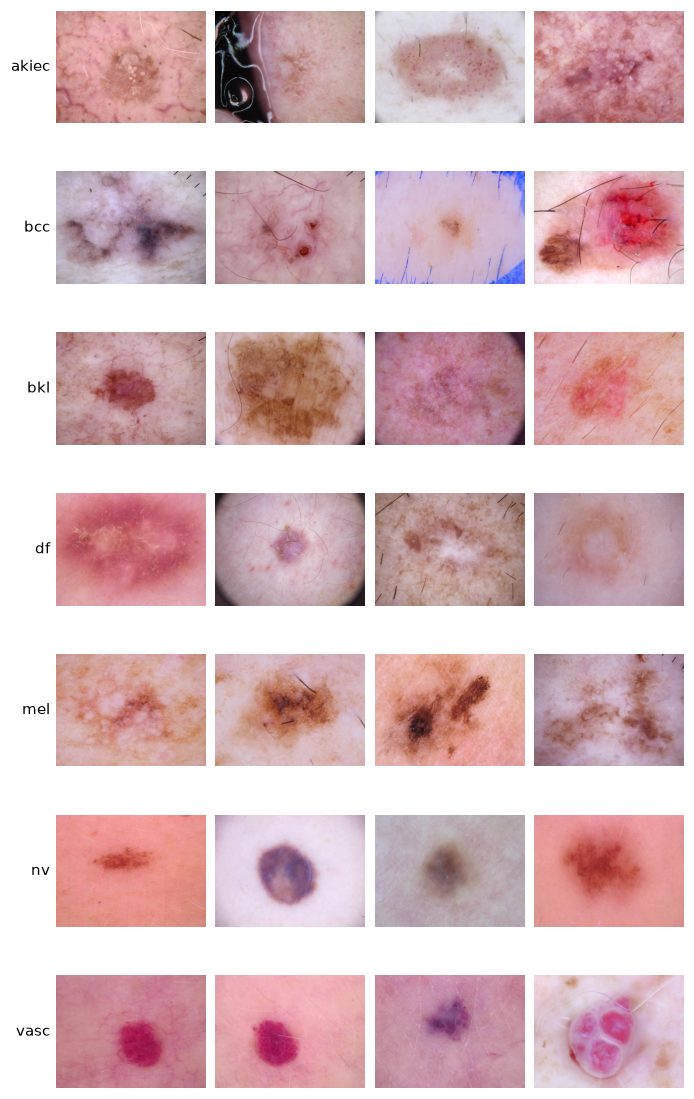
\includegraphics[width=0.6\columnwidth]{figures/samples}
\caption{Random sample images per class, one image per lesion.}
\label{fig:samples}
\end{figure}

\begin{figure}[t]
\centering
% 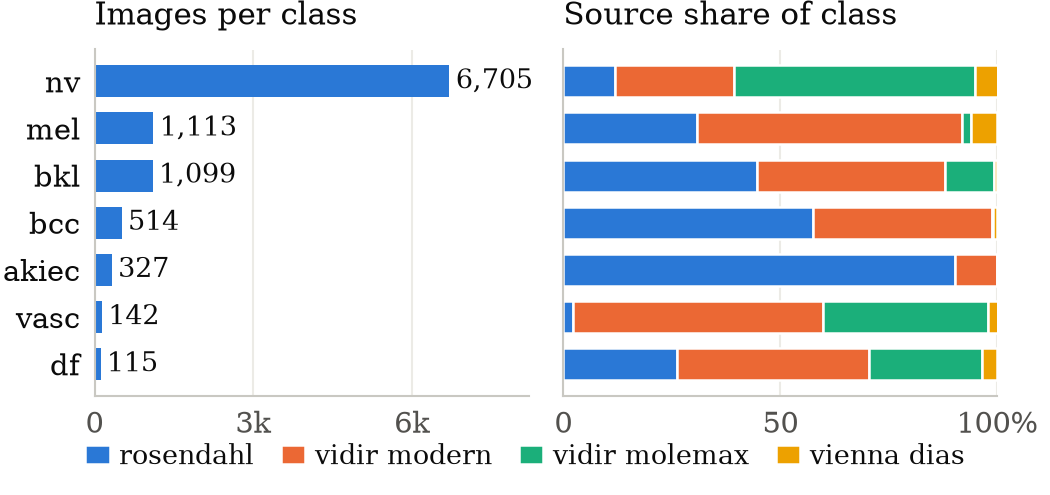
\includegraphics[width=\columnwidth]{figures/class_distribution}
\caption{Label distribution and the share of each class contributed by each source.}
\label{fig:classes}
\end{figure}



\begin{thebibliography}{00}
\bibitem{b1} Esteva, A., Kuprel, B., Novoa, R. et al. Dermatologist-level classification of skin cancer with deep neural networks. \textit{Nature} \textbf{542}, 115--118 (2017). \url{https://doi.org/10.1038/nature21056}
\bibitem{b2} Tschandl, P., Rosendahl, C. \& Kittler, H. The HAM10000 dataset, a large collection of multi-source dermatoscopic images of common pigmented skin lesions. \textit{Scientific Data} \textbf{5}, 180161 (2018). \url{https://doi.org/10.1038/sdata.2018.161}
\bibitem{b3} Kassem, M. A., Hosny, K. M., Damaševičius, R. \& Eltoukhy, M. M. Machine learning and deep learning methods for skin lesion classification and diagnosis: A systematic review. \textit{Diagnostics} \textbf{11}(8), 1390 (2021). \url{https://doi.org/10.3390/diagnostics11081390}
\bibitem{b4} Saputra, V. A., Devi, M. S. K., Diana \& Kurniawan, A. Comparative analysis of convolutional neural networks and vision transformers for dermatological image classification. \textit{Procedia Computer Science} \textbf{245}, 879--888 (2024). \url{https://doi.org/10.1016/j.procs.2024.10.315}
\bibitem{b5} Aruk, I., Pacal, I. \& Toprak, A. N. A comprehensive comparison of convolutional neural network and visual transformer models on skin cancer classification. \textit{Computational Biology and Chemistry} \textbf{120}, 108713 (2026). \url{https://doi.org/10.1016/j.compbiolchem.2025.108713}
\bibitem{b6} Mahbod, A., Tschandl, P., Langs, G., Ecker, R. \& Ellinger, I. The effects of skin lesion segmentation on the performance of dermatoscopic image classification. \textit{Computer Methods and Programs in Biomedicine} \textbf{197}, 105725 (2020). \url{https://doi.org/10.1016/j.cmpb.2020.105725}
\bibitem{b7} Ecer, N., Kankılıç, A. T., Karakoyun, Ö. et al. Diagnostic performance and energy consumption of deep learning models for dermoscopic image classification. \textit{Discover Artificial Intelligence} \textbf{6}, 1530 (2026). \url{https://doi.org/10.1007/s44163-026-02558-5}
\bibitem{b8} Fiaz, M., Shoaib Khan, M. B., Khan, A. H., Bilal, A., Abdullah, M., Darem, A. A. \& Sarwar, R. An explainable hybrid deep learning framework for precise skin lesion segmentation and multi-class classification. \textit{Frontiers in Medicine} \textbf{12}, 1681542 (2025). \url{https://doi.org/10.3389/fmed.2025.1681542}
\end{thebibliography}


\end{document}
